%%%%%%%%%%%%%%%%%%%%%%%%%%%%%%%%%%%%%%%%%%%%%%%%%%%%%%%%%%%%%%%%%%%%%%%%%%%%%%%%%%%%%%%%%%%%%%%%%%%%%%%%%%%%%%%%%%%%%%%%%%%%%%%%%%%%%%%%%%%%%%%%%%%%%%%%%%%
% This is just an example/guide for you to refer to when submitting manuscripts to Frontiers, it is not mandatory to use Frontiers .cls files nor frontiers.tex  %
% This will only generate the Manuscript, the final article will be typeset by Frontiers after acceptance.   
%                                              %
%                                                                                                                                                         %
% When submitting your files, remember to upload this *tex file, the pdf generated with it, the *bib file (if bibliography is not within the *tex) and all the figures.
%%%%%%%%%%%%%%%%%%%%%%%%%%%%%%%%%%%%%%%%%%%%%%%%%%%%%%%%%%%%%%%%%%%%%%%%%%%%%%%%%%%%%%%%%%%%%%%%%%%%%%%%%%%%%%%%%%%%%%%%%%%%%%%%%%%%%%%%%%%%%%%%%%%%%%%%%%%

%%% Version 3.4 Generated 2018/06/15 %%%
%%% You will need to have the following packages installed: datetime, fmtcount, etoolbox, fcprefix, which are normally inlcuded in WinEdt. %%%
%%% In http://www.ctan.org/ you can find the packages and how to install them, if necessary. %%%
%%%  NB logo1.jpg is required in the path in order to correctly compile front page header %%%

\documentclass[utf8]{frontiersSCNS} % for Science, Engineering and Humanities and Social Sciences articles

\usepackage{amsmath,amssymb,booktabs,url,hyperref,lineno,listings,microtype,subcaption}

% Automatic formatting of SI units
\usepackage[binary-units]{siunitx}

\usepackage[onehalfspacing]{setspace}

% Required for 'straight' quotes in code listings
\usepackage[T1]{fontenc}

% Visible TODO notes
\newcommand{\todo}[1]{\textbf{\textsc{\textcolor{red}{(TODO: #1)}}}}

\lstset{language=C++,showstringspaces=false,basicstyle=\tiny,upquote=true,identifierstyle=\ttfamily\color{black}}

\linenumbers


% Leave a blank line between paragraphs instead of using \\


\def\keyFont{\fontsize{8}{11}\helveticabold }
\def\firstAuthorLast{Knight and Nowotny} %use et al only if is more than 1 author
\def\Authors{James C Knight\,$^{1,*}$, Thomas Nowotny\,$^{1}$}
% Affiliations should be keyed to the author's name with superscript numbers and be listed as follows: Laboratory, Institute, Department, Organization, City, State abbreviation (USA, Canada, Australia), and Country (without detailed address information such as city zip codes or street names).
% If one of the authors has a change of address, list the new address below the correspondence details using a superscript symbol and use the same symbol to indicate the author in the author list.
\def\Address{$^{1}$Centre for Computational Neuroscience and Robotics, School of Engineering and Informatics, University of Sussex, Brighton, United Kingdom }
% The Corresponding Author should be marked with an asterisk
% Provide the exact contact address (this time including street name and city zip code) and email of the corresponding author
\def\corrAuthor{James C Knight}

\def\corrEmail{J.C.Knight@sussex.ac.uk}


\begin{document}
\onecolumn
\firstpage{1}

\title[Running Title]{Article Title} 

\author[\firstAuthorLast ]{\Authors} %This field will be automatically populated
\address{} %This field will be automatically populated
\correspondance{} %This field will be automatically populated

\extraAuth{}% If there are more than 1 corresponding author, comment this line and uncomment the next one.
%\extraAuth{corresponding Author2 \\ Laboratory X2, Institute X2, Department X2, Organization X2, Street X2, City X2 , State XX2 (only USA, Canada and Australia), Zip Code2, X2 Country X2, email2@uni2.edu}


\maketitle


\begin{abstract}

%%% Leave the Abstract empty if your article does not require one, please see the Summary Table for full details.
\section{}
While neuromorphic systems may be the ultimate platform for \textit{deploying} spiking neural networks~(SNNs), their distributed nature and optimisation for specific types of models makes them unwieldy tools for \textit{developing} SNN models.
Instead, development and simulation of SNN models tend to be performed on computers or clusters of computers with standard Von Neumann CPU architectures.
Over the last decade, as well as becoming a common fixture in many workstations, NVIDIA GPU accelerators have entered the High Performance Computing field and are now used in \SI{50}{\percent} of the Top 10 super computing sites worldwide.
In this paper we use our GeNN code generator to re-implement two circuit-scale point neuron network models inspired by the neo-cortex on GPU hardware.
We verify the correctness of our GPU simulations against prior results obtained with NEST running on traditional HPC hardware and compare the performance with respect to speed and energy consumption against published data from CPU-based HPC and neuromorphic hardware.
A full-scale model of a cortical column can be simulated at speeds approaching $0.5\times$ real-time using a single NVIDIA Tesla V100 accelerator -- faster than is currently possible using a CPU based cluster or the SpiNNaker neuromorphic system.
In addition, we find that, across a range of GPU systems, the energy to solution as well as the energy per synaptic event of the microcircuit simulation is as much as $14\times$ lower than either on SpiNNaker or in CPU-based simulations.
Besides performance in terms of the speed and energy consumption of the actual simulation, it has recently been identified that efficient initialisation of simulations can be crucial for the utility of different hardware substrates, in particular in a research context where repeated runs and parameter-space exploration are required. 
In this paper we therefore also introduce the novel parallel initialisation methods of GeNN and demonstrate how they afford further speed and energy advantages.

\tiny
 \keyFont{\section{Keywords:} GPU, high-performance computing, parallel computing, accuracy of simulation, energy to solution, benchmarking, computational neuroscience} %All article types: you may provide up to 8 keywords; at least 5 are mandatory.
\end{abstract}

\section{Introduction}
Currently, the most common way to accelerate large-scale spiking neural network (SNN) simulations is to use CPU-based HPC clusters running software simulators such as NEST~\citep{Gewaltig2007} or parallel Neuron~\citep{carnevale2006neuron}.
However, spiking neural networks simulations have a large amount of \textit{fine-grained} parallelism \todo{I realise that I actually have no understanding what ``fine-grained'' referes to here?} which parallel CPU programming paradigms such as multithreading are not well-suited to exploiting.
Furthermore, although the timestep based updates of neuron and synapse dynamics are trivially parallelisable, simulating an SNN also involves the low-latency propagation of spike events between neurons along synaptic connections which is not a good match for standard interconnect protocols such as MPI.

Neuromorphic systems use dedicated hardware, inspired by aspects of the brain, to address the problems of parallelism and efficient spike communication.
The SpiNNaker system~\citep{Furber2014}, developed as part of the Human Brain project (HBP) in Manchester, is a neuromorphic computer consisting of up to a million ARM cores, connected with an interconnect topology optimised for spike-like communication.
The BrainScaleS system developed within HBP at Heidelberg~\citep{Schemmel2017}, uses analog circuit elements rather than digital processors, to emulate the dynamics of point neurons.
Spikes then propagate between these circuit elements through a digital interconnect network.
Other neuromorphic systems based on various combinations of digital and analog hardware include the Loihi chip~\citep{Davies2018} developed by Intel, the TrueNorth chip~\citep{Merolla2014} built by IBM and the Dynapse system~\cite{Qiao2015} developed at University of Zurich.

While neuromorphic systems offer significant theoretical advantages in terms of power efficiency and simulation speed, this often comes at the expense of flexibility.
In systems where physical circuit elements are used to model individual neurons and synapses, the most obvious restriction is that the physical circuits dictate what neuron and synapse models are supported.
Furthermore, in neuromorphic systems of this type, these circuits are instantiated in a fixed ratio (for example 64k synapses to 256 neurons) meaning that Liebig's law dictates that their scalability is limited by the availability of the scarcest of these circuits.
Even fully-programmable systems such as SpiNNaker suffer from this issue as, for example, handling high incoming spike rates consumes a large number of CPU cycles, reducing the number of neurons that can be simulated on each core.
Some of these issues are illustrated in a recent publication by \citet{VanAlbada2018} who investigated the comparative performance of simulations of a micro-column model~\citep{Potjans2012} in NEST-based simulations on an HPC cluster and an implementation on the SpiNNaker neuromorphic system.
This model required smaller simulation timesteps and denser connectivity than SpiNNaker was designed for meaning that, although SpiNNaker achieved the same accuracy as the HPC system, it had to be run $20\times$ slower than realtime with only a small number of neurons simulated on each core. 
Running the model this slowly meant that the theoretical energy and performance advantages of using the SpiNNaker system -- which had been previously demonstrated using models more specifically tuned to it's characteristics~\citep{Sharp2012,Sharp2014,Knight2016} -- were lost and the model not only ran faster on the HPC system but also consumed less energy.
%This was not only slower than NEST running on HPC which achieved runtimes of $3\times$ slower than realtime, but also meant
%The lowest energy consumption for NEST was achieved with \num{144} parallel threads when it ran at $4.6\times$ slower than realtime. 
%At this speed SpiNNaker and NEST consumed about the same energy of \SI{6}{\micro\joule} per simulated synaptic event.

Besides measuring the performance in terms of simulation speed, \citet{VanAlbada2018} also identified that \textit{initialising} and loading large-scale models onto neuromorphic systems efficiently remains a computational challenge. 
For example, the cortical microcircuit model developed by \citet{Potjans2012} took \SI{10}{\hour} to initialise and load onto SpiNNaker.
This confirms earlier observations~\citep{Diamond2018} that prototype neuromorphic systems are not efficient at accelerating their initialisation: Both SpiNNaker and a previous generation of the BrainScaleS system spent a significant amount of time and energy initialising network models on a host machine. 

These factors suggest that when \textit{developing} SNNs, more flexible accelerators which can accelerate the construction, initialisation and simulation of large-scale SNNs are required.
Field-Programmable Gate Arrays (FPGAs) are devices consisting of a large number of lookup-table based logic blocks, connected using a programmable fabric.
While FPGAs have been used to develop various SNN accelerators~\citep{Moore2012,Wang2018}, \citet{Naylor2013} showed that comparable performance can be obtained by building a more flexible programmable FPGA accelerator. \todo{I don't understand the logic of this sentence}
However, although FPGA-based systems of this sort may have potential as more flexible SNN accelerators, FPGAs are not yet commonplace in workstations and their lack of hardware support for floating point arithmetic makes them ill-suited for simulating some classes of neuron and synapse models. 

Alternatively, GPU architectures are designed for high throughput applications with large amounts of fine-grained parallelism.
They swap the large coherent caches, relied upon by modern CPU architectures to improve performance, for large numbers of vector floating point arithmetic units connected to high-bandwidth external memory. 
While originally designed for embarassingly parallel graphics processing, GPU acceleration has also provied to be a good fit for accelerating the training of deep learning systems and is used extensively in modern AI systems. 
The application of GPU acceleration to SNN simulations is also promising and there are a number of active SNN simulator projects which target GPUs. 
Carlsim~\citep{Chou2018} is a C++ based simulator running on NVIDIA CUDA with similar goals as GeNN but is not based on code generation and hence less flexible in the types of models it can support.
EDLUT~\citep{Garrido2011} was initially an event-driven CPU based simulator for SNNs, but has evolved into a hybrid CPU/GPU system with support for both time and event-driven models.
ANNarchy~\citep{Vitay2015} is a code generation based simulator which translates Python model descriptions into multi-core CPU or GPU code with a focus on hybrid rate- and spiking models.
Other simulators that have seen less development in the last 2-4 years include NCS6~\citep{Hoang2013}, Myriad~\citep{Rittner2016}, and NeMo~\citep{Fidjeland2009} (see \citet{Brette2012} for a review).
GeNN \citep{Yavuz2016} is a code-generation library aimed at facilitating accelerated SNN simulations on GPU hardware.
It has been designed to strike a balance between flexibility -- allowing users to define their own model neurons and synapses -- and efficiency in generating optimised CUDA code for the less obviously parallelisable phases of parallel SNN simulations such as spike propagation.

In this paper we introduce novel methods for parallel initialisation of SNNs in the GeNN simulator and investigate the performance of a GPU based simulation in GeNN of the micro-column network model \cite{Potjans2012,VanAlbada2018} as well as a model using STDP in a highly connected network~\citep{Morrison2007}.
We then compare to other recent benchmarks of the models \citep{VanAlbada2018} and critically discuss the current state of the art for SNN simulations.

\section{Material and Methods}
\label{sec:method}
\subsection{GeNN}
\label{sec:method/genn}
As described by \citet{Yavuz2016}, GeNN is a code-generation based system that generates model- and platform-optimised CUDA (Compute Unified Device Architecture \cite{CUDA}) code for GPU accelerated SNN simulations.
In brief, GeNN neuron models are defined by writing a class defining the model parameters and snippets of C-like code that describe how it should be simulated.
For example the following \lstinline{LIF} class describes a leaky integrate-and-fire neuron with normalised units, solved algebraically:

\lstinputlisting[firstline=2,lastline=15]{code_snippets.cc}

The \lstinline{DECLARE_MODEL} and \lstinline{IMPLEMENT_MODEL} macros insert boilerplate code used subsequently for defining parameters and initial model states in a type-safe manner.
The \lstinline{SET_SIM_CODE}, \lstinline{SET_THRESHOLD_CONDITION_CODE} and \lstinline{SET_RESET_CODE} macros specify the snippets of code used, respectively, to update the simulation state, check whether a spike should be emitted and to reset the neuron after a spike.
The names of model parameters (constant across the entire population) are specified using the \lstinline{SET_PARAM_NAMES} macro and any `pre-processing' logic to be applied to these is specified with \lstinline{SET_DERIVED_PARAMS} -- in this case converting an exponential decay time constant to a multiplier to be applied every simulation timestep.
Finally, the \lstinline{SET_VARS} macro specifies the names and types of the per-neuron state variables.
These macros provide some `syntactic sugar' but are entirely optional -- users can instead override the underlying virtual functions themselves.
In GeNN, synapse models are defined using very similar classes with the option to define code snippets for time-driven and event-driven updates.
Event-driven updates can be triggered by pre or postsynaptic spikes as well as by custom events for example the pre or postsynaptic neuron's membrane voltages crossing a threshold.
Once the required models have been defined, the values of parameters and initial state variables can be set and \textit{populations} of neurons can be added to a network:
%
\lstinputlisting[firstline=17,lastline=20]{code_snippets.cc}

This listing also illustrates how the approach used for defining models now can also be used to define how variables are initialised, a new mechanism added since GeNN 3.xx:
The membrane voltage \lstinline{V} of our \num{1000} LIF neurons is sampled from the uniform distribution using one of GeNN's built in \textit{variable initialisation snippets}, which are definied in a similar manner to the neuron and synapse code snippets. Using this mechanism allows GeNN to parallelise network initialisation employing the same parallelisation strategies for initialisation on the GPU as for simulating the models.
This approach is advantageous as it both, removes the need to transfer the model state from the CPU to the GPU and allows the GPU to be used to accelerate potentially costly initialisation operations such as sampling random numbers.

Once network models have been defined using the C++ interface, GeNN will generate the CUDA code to initialise and simulate the network which can then be linked against a simulation loop provided by the user:

\lstinputlisting[firstline=22,lastline=32]{code_snippets.cc}

While this approach allows a lot of flexibility and means that visualisation tools and closed-loop robotics can be tightly coupled to GeNN simulations, when combined with the use of C++ for model definition, this does make using GeNN a somewhat daunting prospect to users more used to Python-based simulators such as Brian~\citep{Stimberg2014} or PyNN~\citep{Davison2008a} or graphical tools such as SpineCreator~\citep{Cope2017}.
For these users, GeNN can be used as a backend for other other simulators.
Brian2GeNN~\citep{Stimberg2018} allows models to be defined in Brian 2 and it translates them using code generation into a valid GeNN simulation. 
Using Brian 2's backend device design, using GeNN through Brian2GeNN is as simple as issuing the command \lstinline[language=python]{set_device("brian2genn")} within a standard Brian 2 script. 
A similar interface exist for SpineCreator and an interface to PyNN~\citep{Davison2008a} is currently being developed.

\subsection{The cortical microcircuit model}
\label{sec:method/microcircuit}
This model of \SI{1}{\milli\metre\cubed} of early-sensory cortex was developed by \citet{Potjans2012} and consists of around \num{80000} neurons, divided into layers 2/3, 4, 5 and 6.
Each layer is modelled by an excitatory and an inhibitory neuron population.
Neurons in each population are connected randomly with population-specific densities derived from an extensive review of the anatomical literature resulting in a total of approximately \num{0.3E9} synapses.
For a full description of the model please refer to \citeauthor{Potjans2012}.
In the remainder of the this section we will concentrate on describing the strategies used to parallelise the initialisation and subsequent simulation of this network.

In this model the density of the synaptic connections between a pair of neuronal populations is specified in terms of a total number of random synapses (a \lstinline{FixedNumberTotal} connector in PyNN).
The first stage in initialising such a connectivity between a presynaptic population with $N_{\text{pre}}$ neurons and a postsynaptic population with $N_{\text{post}}$ neurons is to determine how many of the total synapses $N$ end up in each row by sampling from the multinomial distribution $\text{Mult}[N_{\text{pre}} * N_{\text{post}}, \{P_{row}, P_{row}, \ldots, P_{row}\}]$ where $P_{row} = \frac{N_{\text{post}}}{N}$.
This operation cannot be efficiently parallelised so must be performed on the host but, once the length of each row is determined, the postsynaptic targets of the synapses can be initialised in parallel by sampling from the discrete uniform distribution $\text{Unif}[0, N_{\text{post}}]$ parallelised across $N_{\text{pre}}$ CUDA threads.
However, although this works mathematically, so as to improve the locality of memory accesses, synapses should be sorted into ascending order.
This would be trivial to implement in CPU code but, without enough shared memory for each CUDA thread to store a copy of its corresponding row, an in-place sort in global memory would be very slow.
It would be possible to use a more complex parallel sorting algorithm such as that proposed by \citet{Awan2016} but, as GPU architectures typically have very high floating point maths throughput, we instead take an alternative approach.
Rather than sampling directly from $\text{Unif}[0, N_{\text{post}}]$ we sample from its 1st order statistic $\text{Beta}[1, N_{\text{post}}]$ -- essentially the next smallest value.
In the general case the Beta distribution cannot be sampled from in constant time.
However, if $X \sim \text{Beta}[1, N_{\text{post}}]$, $1 - X \sim \text{Beta}[N_{\text{post}}, 1]$ and $-ln(1 - X) \sim \text{Exponential}[N_{\text{post}}]$ -- a much simpler problem as the exponential distribution can be sampled in constant time using the inversion method~\citep{DevroyeLuc2013}.

Beside this structured connectivity, all synaptic strengths and transmission delays are normally distributed.
In addition to their synaptic input, each neuron in the network also receives independent Poisson inputs with population-specific rates representing input from adjacent cortical regions.
Neurons are modelled as leaky integrate-and-fire~(LIF) units with exponentially shaped current inputs:
%
\begin{align}
    \tau_{m} \frac{dV_{j}}{dt} = & (V_{j} - V_{rest}) + R_{m}(I_{bias} + I_{s_{j}}) \label{eq:lif_neuron}\\
    \tau_{syn} \frac{dI_{s_{j}}}{dt} = & -I_{s_{j}} + \sum_{i=0}^{n} w_{ij} \sum_{t_{i}^{f}}  \delta(t - t_{i}^{f})\label{eq:exp_neuron_input_current}
\end{align}
%
Although $V_{j}$ and $I_{s{j}}$ are coupled, in our GeNN model, the continuous terms of the two equations are solved separately such that the synaptic input current $I_{s_{j}}$ going into equation~\ref{eq:lif_neuron} is effectively treated as a constant during each simulation timestep.
As \citet{Rotter1999} explain, this approach leads to a delay of one simulation timestep compared to the exact solution.
However, by separating the solving of these equations, different types of input synapse with different dynamics can be trivially supported.
For example, while a single exponential may be a good approximation of some inhibitory synapses, for other types of synapse the rise time of the post synaptic potential may be vital~\citep{VanVreeswijk1994}.
Additionally, from a software engineering point-of-view, separating the solving of these equations improves the encapsulation of neurons and synapses.

Simulating a homogeneous \textit{population} of neurons is an ideal task for a SIMD or SIMT device such as a GPU: the neurons do not communicate with each other and, aside from the relatively rare times that they spike, each neuron will be running exactly the same code.
This means that they can be trivially parallelised by simulating each neuron on a single thread which fetches the neuron's state variables from global memory into registers at the start of each timestep, then advances the simulation state and writes back the state variables.
As long as the state variables are laid out correctly in memory, the required memory operations can be \textit{coalesced} so that a \SI{4}{\byte} state variable can be read for \num{32} neurons in a single \SI{128}{\byte} transaction -- the most efficient way to access the global memory.
%This same parallelism strategy is equally valid for neuron models whose dynamics can only be solved numerically -- the advancing of simulation state simply has to be implemented as for example a Runge-Kutta

\begin{figure}
    \begin{center}
        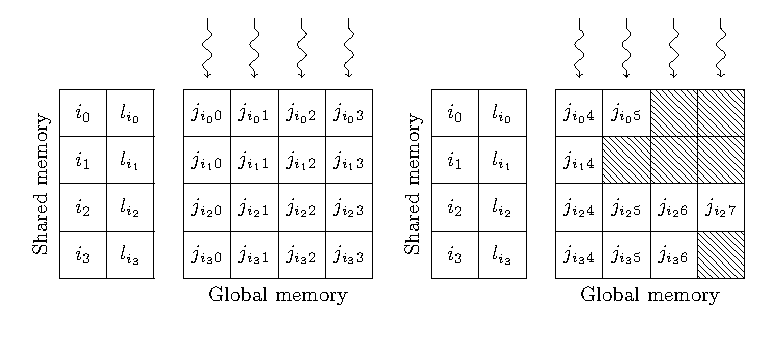
\includegraphics[width=118mm]{figures/ragged_matrix}
    \end{center}
    \caption{GPU parallelism of sparse synaptic matrix processing across two thread blocks each with \num{4} threads.
    Snaking lines indicate CUDA threads.
    Hatching indicates padding entries.}
    \label{fig:ragged_matrix}
\end{figure}

Simulating the sparsely connected synapses between two such populations of neurons is, at first glance, less suitable for GPU parallelism.
However, on modern GPU hardware, this can also be implemented in an efficient manner using the data structures shown in figure~\ref{fig:ragged_matrix}.
This structure consits of multiple 2D arrays where each row represents the synapses coming from a single presynaptic neuron and has enough columns to contain the largest number of postsynaptic targets any presynaptic neuron connects to.
One of these 2D arrays is used to contain the indices of the postsynaptic neurons ($i$) and additional arrays are allocated for any individual synaptic state variables such as the synaptic weight~($w_{ij}$) or dendritic delay~($d_{ij}$).
Each block of $N_{block}$ CUDA threads (in figure~\ref{fig:ragged_matrix} $N_{block}=4$) is responsible for processing $N_{block}$ columns of the matrix.
Processing begins by using the $N_{block}$ threads to fetch the indices of $N_{block}$ presynaptic spikes ($i_{0},\ldots,i_{N_{block} - 1}$) and the lengths of the corresponding rows of the matrix ($l_{0},\ldots,l_{N_{block} - 1}$) into shared memory (as these will be accessed by all threads in the block during the next phase).
Threads are then synchronised and loop through the $N_{block}$ rows with each thread processing the synapse in their column.
In the case of the simple static synapses described by equation~\ref{eq:exp_neuron_input_current} this processing consists simply of reading the index of the postsynaptic target neuron along with the weight $w_{ij}$ and delay $d_{ij}$ associated with the connection and using an atomic add operation to apply the weight to the correct address in the dendritic delay ring-buffer.\todo{say more}
This process is then repeated until all incoming spikes are processed.
While this parallelism strategy may seem counter-intuitive, it typically performs much better than the naïve approach of using one thread per incoming spike as it exposes much more parallelism as well as resulting in perfectly coalesced memory read operations.
For example, if we consider a population of \num{10000} neurons firing at an average rate of \SI{10}{\hertz}, in a \SI{0.1}{\milli\second} timestep it will only, on average, emit \num{10} spikes in a single timestep.
However, if this population is connected to another population with the same size with a \SI{10}{\percent} connection probability, the connection matrix will have over \num{1000} columns resulting in 2 orders of magnitude more parallelism being exposed.

\subsection{Balanced random network with spike-timing dependant plasticity}
\label{sec:method/balanced_random}
The type of one-shot, online learning observed in nature is one of the features of biological neural networks that neuromorphic engineers aspire to emulate.
Synaptic plasticity -- the family of mechanisms responsible for changing the strength of synaptic connections in response to neural activity -- has been shown to be fundamental to learning~\citep{Nabavi2014} and is therefore a key area of computational neuroscience research.
Spike Timing Dependant Plasticity~(STDP)~\citep{Bi1998} is a popular theory which postulates that these changes are driven by the difference in timing between presynaptic spikes arriving at a synapse and the times at which the postsynaptic neuron itself spikes.
In excitatory cortical neurons~\citep{Markram1997} as well as in the Hippocampus~\citep{Bi1998}, synapses at which a presynaptic spike is closely followed by a postsynaptic spike are strengthened, whereas those at which a postsynaptic spike precedes a presynaptic spike are weakened.
The intuition behind this relationship is that synapses that are implicated in the firing of the postsynaptic neuron are strengthened and those that are irrelevant are weakened.

However, adding STDP to spiking neural network simulations typically increases the computational cost of simulating them significantly. 
\citet{Morrison2007} reported that adding plasticity to their simulations slowed them down by ``a factor of less than 10'' and \citet{Knight2016b} found that, in the \textbf{best} case, simple STDP plasticity reduced the performance of the SpiNNaker neuromorphic system by approximately $6\times$.
Furthermore, the dynamics of neural systems with plasticity operating on biologically-plausible time scales take several orders of magnitude more time to stabilise.
%Perhaps because of these issues, there are relatively few large-scale network models with synaptic plasticity.
However, \citeauthor{Morrison2007} argue that it is vital to perform experiments on STDP in models with full-scale connectivity, as simplifying connectivity typically results in fewer, stronger incoming synapses per neuron.
These stronger synaptic inputs are then likely to increase the correlation between neurons and, because STDP is inherently sensitive to correlated neural activity, this is likely to cause artefacts in the learned synaptic weights.
On this basis, \citeauthor{Morrison2007} developed a large balanced random network model~\citep{Brunel2000} with \num{90000} excitatory and \num{22500} inhibitory neurons, the scale necessary to achieve realistic connection probabilities of $\approx 0.1$ and number of incoming connections per neuron of $\approx 10000$ ~\citep{braitenberg2013cortex}.

When the density of the synaptic connections is described using a probability of connection $P$, whether a synapse exists between a pair of pre and postsynaptic neurons can be modelled using the Bernoulli distribution $\text{Bern}[P]$.
While the Bernoulli distribution can be sampled by repeatedly drawing from the uniform distribution $\text{Unif}[0, 1]$ and comparing each sample to $P$, this is innefficient for sparse connectivity.
Instead we sample from the geometric distribution $\text{Geom}[P]$ which describes how the number of Bernoulli trials required to get a success (i.e. a synapse) is distributed.
The geometric distribution can be sampled in constant time by inverting the CDF of the equivalent continuous distribution (the exponential distribution) to obtain $\frac{log(\text{Unif}[0, 1])}{log(1 - P)}$~\citep{DevroyeLuc2013}.
Using this approach, generating fixed probability connectivity can be performed entirely in parallel by initialising each row of connectivity with an independent CUDA thread.

Balanced random networks have been shown to reproduce some of the dynamics seen in the neocortex~\citep{Brunel1999,Brunel2000} and \citeauthor{Morrison2007} showed that adding STDP to such a network does not disrupt these dynamics and weights remain stable.
For the full description of this model, please refer to \citeauthor{Morrison2007}.
In the remainder of this section we will concentrate on describing how models with synaptic plasticity are parallelised using GeNN.

Similarly to the microcircuit model described in the previous section this model uses LIF neurons with current inputs.
However, rather than exponentially filtering the incoming synaptic input, this model uses slightly more complex \textit{alpha} synapses~\citep{Rall1967} which provide a closer match to the dynamics of biological ion channels:
%
\begin{align}
    \tau_{syn} \frac{dI_{s_{j}}}{dt} = & x_{s_{j}} - I_{s_{j}} \label{eq:alpha_neuron_input_current_1}\\ 
    \tau_{syn} \frac{dx_{s_{j}}}{dt} = & -x_{s_{j}} + \sum_{i=0}^{n} w_{ij} \sum_{t_{i}^{f}}  \delta(t - t_{i}^{f}) \label{eq:alpha_neuron_input_current_2}
\end{align}
%
Aside from requiring an additional state variable to hold $x_{s_{j}}$, equations~\ref{eq:alpha_neuron_input_current_1}~and~\ref{eq:alpha_neuron_input_current_2} have trivial algebraic solutions meaning they can be simulated using the same scheme described in the previous section.

Even leaving aside synaptic plasticity rules which use postsynaptic membrane voltage~\citep{Brader2007,Clopath2010c} rather than postsynaptic spike times or include `third factors' such as dopamine~\citep{Izhikevich2007}, there are a plethora of different STDP formalisations (see \citet{Morrison2008} for a review).
However, in the model described in this section, \citet{Morrison2007} chose to use a rule with the following relationship between pre~($t_{\text{pre}}$) and postsynaptic~($t_{\text{post}}$) spike timing ($\Delta t = t_{\text{post}} - t_{\text{pre}}$):
%
\begin{align}
    \Delta w_{ij} = \
        \begin{cases}
            \lambda w_{0}^{1-\mu} w_{ij}^{\mu} e^{-\frac{|\Delta t|}{\tau}} & if\, \Delta t>0\\
            -\lambda \alpha w_{ij} e^{-\frac{|\Delta t|}{\tau}}             & if\, \Delta t\leq0
        \end{cases}\label{eq:mad_stdp}
\end{align}
%
\citet{Morrison2007} use this rule with an \textit{all-to-all} spike-pairing scheme meaning that each of the pairs formed by a presynaptic spike and all preceding postsynaptic spikes (and vice-versa) should be considered.
Rather than repeatedly evaluating equation~\ref{eq:mad_stdp}, we calculate these updates based on pre and postsynaptic \textit{spike traces}~\citep{Song2000, Morrison2007} with the following dynamics:
%
\begin{align}
    \frac{ds_{i}}{dt} & = -\frac{s_{i}}{\tau} + \sum_{t_{i}^{f}}\delta(t - t_{i}^{f}) \label{eq:stdp_trace}\\
\end{align}
%
These traces are then used to calculate the magnitude of $\Delta w_{ij}$ when a pre or postsynaptic spike arrives at the synapse:
%
\begin{align}
  \Delta w_{ij}^{-}(t_{i}^{f}) & = \lambda \alpha w_{ij} s_{j}(t_{i}^{f})\label{eq:stdp_update_pre_pair}\\
  \Delta w_{ij}^{+}(t_{j}^{f}) & = \lambda w_{0}^{1-\mu} w_{ij}^{\mu} s_{i}(t_{j}^{f})\label{eq:stdp_update_post_pair}
\end{align}
%
In GeNN, if a neuron has fired in the current timestep, its trace variables are updated in the neuron kernel.
Synaptic depression (equation~\ref{eq:stdp_update_pre_pair}) is applied in the synapse kernel described in the previous section.
However applying synaptic potentiation (equation~\ref{eq:stdp_update_post_pair}) is a little more tricky as it needs to be applied to each synapse in the \textbf{column} of the data structure shown in figure~\ref{fig:ragged_matrix} associated with a spiking postsynaptic neuron.
Sparse matrix data structures seldomly support efficient accesses to both rows and columns, making this a problem for many large-scale SNN simulators.

Some small-scale neuromorphic systems have solved this problem in hardware using custom SRAM memories which allow both column-wise and row-wise accesses~\citep{Seo2011}.
However, custom SRAMs are expensive in terms of silicon area, so many neuromorphic systems avoid the problem entirely by implementing synaptic plasticity rules based on the postsynaptic membrane voltage rather than the postsynaptic spike times meaning that  no updates triggered by postsynaptic spikes are required~\citep{Frenkel2018,Qiao2015}.
Intel's Loihi system~\citep{Davies2018} defers all STDP updates triggered by postsynaptic spikes until the end of a ``learning epoch'' after which time they are processed sequentially row by row.
NEST~\citep{Morrison2007} and SpiNNaker~\citep{Knight2016} both buffer postsynaptic spikes until the next presynaptic spike occurs -- allowing weight updates resulting from spikes to be applied in order without having to make any column-wise accesses to the synaptic matrix. 
However this approach makes access to postsynaptic variables difficult as they would need to be buffered for an unbounded length of time until the next presynaptic spike occurs.

Deferring STDP updates ideally requires a dynamic memory structure to store postsynaptic events and, when combined with the subsequent searching within this data structure for events to apply, this approach does not appear to be well suited for GPU implementation.
Furthermore, GeNN aims to support a wide range of synaptic plasticity rules with full access to pre and postsynaptic neuron variables.
Therefore, GeNN builds an additional \textbf{column-wise} sparse matrix using the same data structure shown in figure~\ref{fig:ragged_matrix}, containing indices into the original row-wise arrays containing synaptic weights.
This has the downside of doubling the memory requirements of connections when STDP is required and additionally, as \citet{Yavuz2016} demonstrated, the resultant non-coalesced accesses to the synaptic matrix reduce performance on lower-end GPUs. \todo{say why it's nevertheless the best solution}

\begin{figure}
    \begin{center}
        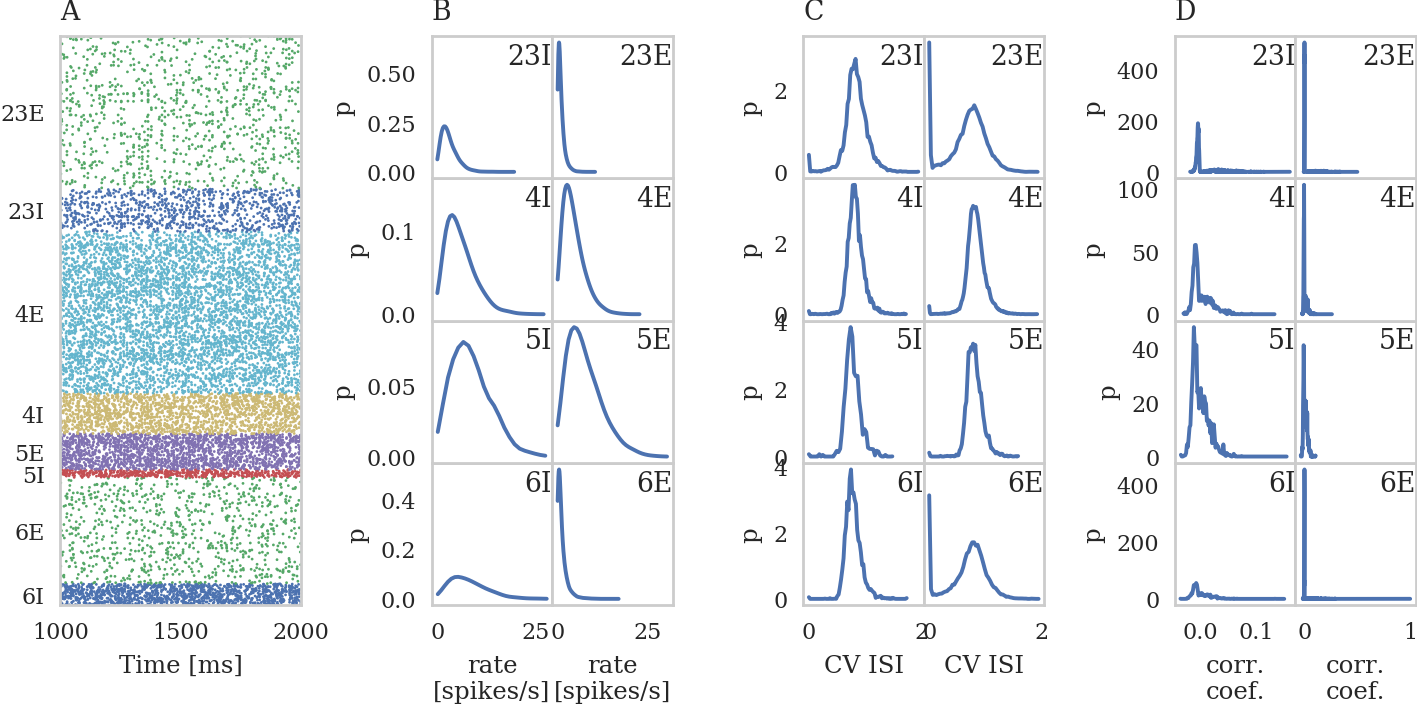
\includegraphics[width=180mm]{figures/microcircuit_accuracy}
    \end{center}
    \caption{Spiking output of cortical microcircuit model with Poisson input.\\
    \textbf{(A)} Raster plot showing spike times (dots) of neurons from each population.
    The spikes of 5\% of neurons (vertical) are shown.\\
    \textbf{(B)} Single-neuron firing rates of all neurons.\\
    \textbf{(C)} CV ISI, a measure of irregularity of all neurons.\\
    \textbf{(D)} Correlation coefficients between binned spike trains for \num{200} neurons in each population.
    All measures are calculated over the last \SI{9}{\second} of the simulation and histogram bin widths are determined using the Freedman-Diaconis rule.}
    \label{fig:microcircuit_accuracy}
\end{figure}

\begin{figure}
    \begin{center}
        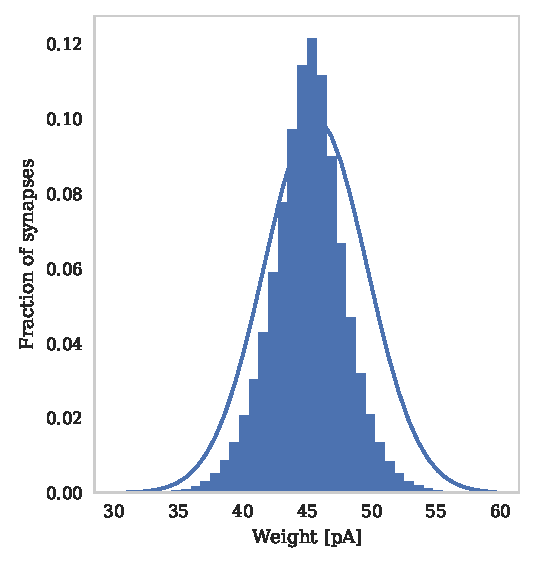
\includegraphics[width=85mm]{figures/mad_weights}
    \end{center}
    \caption{Histogram of the equilibrium synaptic weight distribution calculated after \SI{2000}{\second} of simulation.
    The solid green line shows the gaussian distribution with $\mu_{w} = 46.25$ and $\sigma_{w} = 4.07$.}
    \label{fig:mad_weights}
\end{figure}

% \begin{table}
%   \centering
%   \begin{tabular}{r S S S S S}
%     \toprule
%         {Simulation}         & {Mean weight}             & {Weight standard deviation} & {Mean spike rate} & {Covariance of interspike interval} & {Fano factor}\\
%     \midrule
%         \citet{Morrison2007}    & 45.65 & 4.07 & 8.8 & 0.88 & 8.5\\
%         GeNN                    & 46.25 & 3.99 & 8.8 & 0.86 & 8.3\\
%     \bottomrule
%   \end{tabular}
% 
%   \caption{GPU devices.}
%   \label{tab:mad_stats}
% \end{table}
\begin{table}
  \centering
  \begin{tabular}{r S S}
    \toprule
        {Statistic}                                     & {Value reported by}       & {Value obtained from} \\
                                                        & {\citet{Morrison2007}}    & {GeNN simulation} \\
    \midrule
        Mean weight [\si{\pico\ampere}]                 & 45.65                     & 46.25 \\
        Weight standard deviation [\si{\pico\ampere}]   & 3.99                      & 4.07 \\
        Mean spike rate [\si{\hertz}]                   & 8.8                       & 8.8 \\
        Covariance of interspike interval               & 0.88                      & 0.86 \\
        Fano factor                                     & 8.5                       & 8.3 \\
    \bottomrule
  \end{tabular}

  \caption{Comparison of statistics reported by \citet{Morrison2007} with those obtained from our GeNN simulations.}
  \label{tab:mad_stats}
\end{table}

\section{Results}
\subsection{Correctness}
\label{sec:results/correctness}
\citet{VanAlbada2018} performed an in-depth analysis of the correctness of simulations of the microcircuit model described in section~\ref{sec:method/microcircuit} \citep{Potjans2012}  both on the SpiNNaker neuromorphic system and on NEST running in `grid-based' mode.
The GPU simulations presented in this paper do not face the issues with quantisation which can affect SpiNNaker due to its use of relatively low-precision fixed-point arithmetic.
However, unlike NEST, our GPU simulations use single rather than double-precision floating point and therefore have the potential for more numerical instability.
Additionally, the non-associative nature of floating point operations means that, if the results from a large number of parallel threads are summed together in a non-deterministic order, this can lead to large differences between runs due to rounding errors.
\citet{Villa2009} demonstrated this by calculating the sum of \num{28000} double-precision floating point numbers across \num{16000} threads of a CRAY XMT system (which, in this context, has similar properties to a GPU) and found that results varied by up to \SI{24.64}{\percent}.
However, in this experiment, more numbers were summed than might occur in any of the parallelisation schemes described in section~\ref{sec:method} and it is unclear what absolute errors these reported relative errors correspond to. A more detailed treatment of the expected rounding errors in parallel simulations of SNNs on GPUs will be published elsewhere \citep{Turner2019}. In this section we will focus on confirming the correctness of our simulations using the methodology described by \citet{VanAlbada2018} to compare the results of our microcircuit simulation to those obtained using NEST running in `precise' mode.

While the randomisation of each neuron's initial membrane voltage should reduce any such effects, the first \SI{1}{\second} of spike data from each \SI{10}{\second} simulation is discarded in order to remove any transients.
We then calculated the average firing rates and the covariance of interspike intervals~(CV ISI) for each neuron in the model throughout the remaining \SI{9}{\second} of spiking data using the Elephant~\citep{Yegenoglu2018} package.
We also picked \num{200} (this was a trade-off between accuracy and analysis time chosen by \citeauthor{VanAlbada2018}) active neurons from each population, binned their spike trains into \SI{2}{\milli\second} bins (corresponding to the refractory time of the neurons) and calculated the Pearson correlation coefficients matrix between each disjoint pair of neurons.

The same statistics were calculated from a NEST simulation running in `precise' mode.
Histograms of all three measures were produced using bins calculated with the Freedman-Diaconis rule~\citep{Freedman1981} from the NEST data.
The histograms were smoothed with Gaussian kernel density estimation performed using the \lstinline{scipy.stats.gaussian_kde} function with bandwidths of \SI{0.3}{\per\second}, \num{0.04} and \num{0.002} for the average firing rates, CV ISI and correlation respectively.

Figure~\ref{fig:microcircuit_accuracy} shows the results of this analysis.
Visually it is clear that the per-population distributions are highly similar and, to quantify this, we calculated the Kullback-Leibler~(KL) divergences using the NEST data as the reference.
Similarly to the KL divergences \citet{VanAlbada2018} reported for their grid-aligned NEST and SpiNNaker simulations, the divergence between the distributions from the GeNN simulations and those produced by NEST running in `precise' mode are comparable in size to the divergences caused by simply changing the seed used for random number generation. \todo{Should we sho the corresponding KL values in the figure???}
This suggests that using single-precision floating point and summing inputs in a non-deterministic order has a minimal effect on the dynamics of the microcircuit model.

So as to assess the correctness of our implementation of the balanced random network model described in section~\ref{sec:method/balanced_random}, we simulated the network for \SI{2000}{\second} of biological time and compared the final weight distribution and spike statistics from the last \SI{50}{\second} with those reported by \citet{Morrison2007}.
These statistics are listed in table~\ref{tab:mad_stats} and the final weight distribution is shown in figure~\ref{fig:mad_weights}.
The final weight distribution has a small right skew it is otherwise similar to that reported by \citeauthor{Morrison2007}.
So as to quantify the network dynamics resulting from these synaptic weights, we calculate the mean firing rate and CV ISI of all excitatory neurons in the network.
The mean firing rate and CV ISI values listed in table~\ref{tab:mad_stats} suggest that our model had settled into a very similar asynchronous-irregular regime to that reported by \citeauthor{Morrison2007}.
Our model exhibited fast oscillations throughout the simulation and, to quantify the resultant variation in spike rate, we calculated a histogram with \SI{3}{\milli\second} bins from the output spike trains of \num{1000} excitatory neurons.
By dividing the variance of each bin's spike count by it's mean we calculated a Fano factor which, again, was very simular to that reported by \citeauthor{Morrison2007}.
These statistical differences could be purely numerical -- due to our use of single-precision floating point and CUDA's approximate exponential and power functions -- or because of subtle differences in the synaptic delay model between GeNN and NEST.

\subsection{Performance}
\label{sec:results/performance}
To assess the performance of our GPU simulations we chose the selection of GPUs listed in table~\ref{tab:gpu_devices} -- covering a range of financial and power budgets.
CUDA abstracts away the degree of parallelism exposed by the application from the amount of hardware parallelism available so we can run a model that uses \num{80000} threads on a GPU with many fewer CUDA cores.
However memory is a harder constraint so, while all of the GPUs listed in table~\ref{tab:gpu_devices} can run the microcircuit model described in section~\ref{sec:method/microcircuit}, due to the increased memory requirements of STDP connections, only the two `Tesla' GPUs have enough memory to run the balanced random network model described in section~\ref{sec:method/balanced_random}.

\begin{table}
  \centering
  \begin{tabular}{r S r S S S S}
    \toprule
        {Model}         & {TDP}             & {Architecture}    & {Num.}    & {Memory}              & {Memory}                      & {Max single-precision}\\
                        & {[\si{\watt}]}    &                   & {CUDA}    & {capacity}            & {bandwidth}                   & {performance}\\
                        &                   &                   & {cores}   & {[\si{\giga\byte}]}   & {[\si{\giga\byte\per\second}]}& {[GFLOPS]}\\
    \midrule
        GeForce 1050 Ti & 75                & Pascal            & 768       & 4                     & 112                           & 2100\\
        Jetson TX2      & 15                & Pascal            & 256       & 8\textsuperscript{1}  & 58.4                          & 750\\
        Tesla K40c      & 235               & Kepler            & 2880      & 12                    & 288                           & 4290\\
        Tesla V100      & 250               & Volta             & 5120      & 16                    & 900                           & 14000\\
    \bottomrule
  \end{tabular}

  \caption{GPU devices.\\
  \textsuperscript{1}~Memory is shared between CPU and GPU.}
  \label{tab:gpu_devices}
\end{table}

\begin{figure}
    \begin{center}
        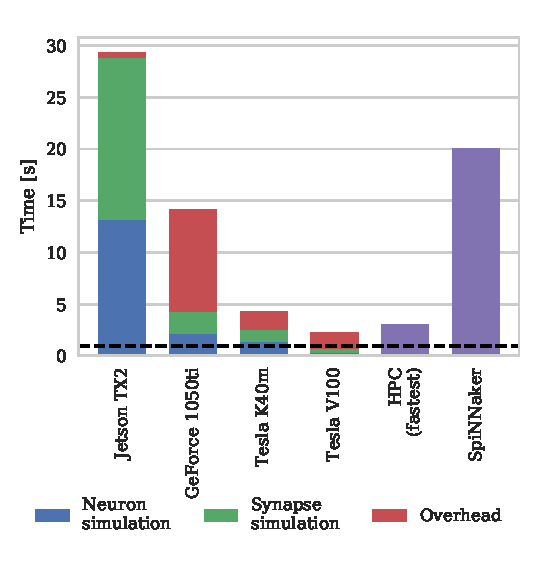
\includegraphics[width=85mm]{figures/microcircuit_performance}
    \end{center}
    \caption{Simulation times of microcircuit model running on various GPU hardware for \SI{10}{\second} of biological time.
    SpiNNaker and fastest HPC simulation times (12 nodes) presented by \citet{VanAlbada2018} included for comparison.
    `Overhead' in GPU simulations refers to time spent in simulation loop but not within CUDA kernels.}
    \label{fig:microcircuit_performance}
\end{figure}

\begin{figure}
    \begin{center}
        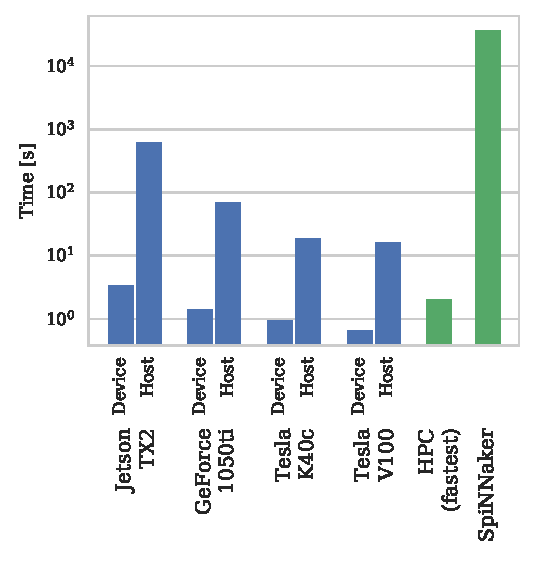
\includegraphics[width=85mm]{figures/microcircuit_init_performance}
    \end{center}
    \caption{Initialisation times of microcircuit model running on various GPU hardware.
    SpiNNaker and fastest HPC simulation times (32 nodes) presented by \citet{VanAlbada2018} included for comparison.}
    \label{fig:microcircuit_init_performance}
\end{figure}

We measured the performance of both models by querying the \lstinline{std::chrono::high_resolution_clock} on the host computer around the simulation loop to get a total simulation time and, in the case of the microcircuit model, around the code used to calculate the connectivity.
Additionally we used CUDA's own event timing system~\citep[Section~8.1.2]{NVIDIACorporation2018} to record the time taken by the neuron and synapse simulation kernels as well as the postsynaptic learning kernel in the balanced random network model.

Figure~\ref{fig:microcircuit_performance} shows the durations of simulations of the microcircuit model running on each GPU for \SI{10}{\second} of biological time, including the times taken by neuron and synapse simulation kernels.
Compared to the smaller point neuron benchmark presented by \citet{Yavuz2016}, even though each neuron in our model receives up to $10\times$ as many synaptic inputs, the simulation time is more evenly split between the simulation of neurons and synapses.
This is partly because our simulations are running with a smaller \SI{0.1}{\milli\second} timestep meaning that less presynaptic spikes are processed each timestep.
Additionally, in the newer version of GeNN used in this paper, the generation of Poisson noise takes place in the neuron kernel rather than in the separate kernel used by \citeauthor{Yavuz2016}.

In general, as one would expect, the two Tesla GPUs perform best with the newer Tesla V100 system achieving a faster simulation speed than was possible on the CPU-based HPC cluster \citep{VanAlbada2018}.
However even the GeForce 1050ti, which is a low-end gaming GPU, can simulate the model faster than the SpiNNaker system although this system has a much higher overhead than any of the other GPUs.
We believe that this overhead is likely to be due to a combination of the slower PCI express bus in this machine (PCIe Gen 2 rather than Gen 3) and issues using CUDA on display devices under Windows.

Because the Jetson TX2 is a system-on-chip in which the CPU and GPU cores share the same physical memory, the same blocks of memory can be directly accessed from both CPU and GPU code.
Therefore, unlike on the other GPU systems benchmarked, spike recording can be implemented without copying data from the GPU to the CPU every time step.
We believe that this is the reason that the `overhead' of the simulation running on the Jetson TX2 is significantly smaller than on any of the other systems.

As discussed in section~\ref{sec:method/genn}, as well as parallelising neuron and synapse simulation code, GeNN also parallelises the initialisation of model state variables and connectivity using the GPU.
Figure~\ref{fig:microcircuit_init_performance} shows the initialisation time of the microcircuit simulation when initialisation is performed on the CPU compared to the GPU.
Even on the two Tesla systems which have powerful Intel Xeon CPUs with high single-thread performance, using the GPU for initialisation, results in a speedup of around $20\times$.
Furthermore, on the Jetson TX2 with its much slower ARM A57 CPU, GPU initialisation is more than $150\times$ faster.

Figure~\ref{fig:microcircuit_init_performance} also includes the initialisation times for SpiNNaker and the fastest HPC configuration presented by \citeauthor{VanAlbada2018}.
The scaling plot for HPC initialisation confirms the trivially parallelisable nature of network initialisation compared to simulation.
Performance continues to increase up to using 32 nodes rather than only 12 in the simulation.
However, all three desktop GPU systems still perform network initialisation in a shorter time than the HPC system.
\citet{Diamond2018} concluded that initialisation and loading time was a big problem for neuromorphic systems and SpiNNaker clearly still has issues in this area.
Initialising the microcircuit network and loading it onto the SpiNNaker system takes approximately \SI{10}{\hour} which is approximately $50\times$ slower than the Jetson TX2 when only a single ARM core is used for initialisation.

\begin{figure}
    \begin{center}
        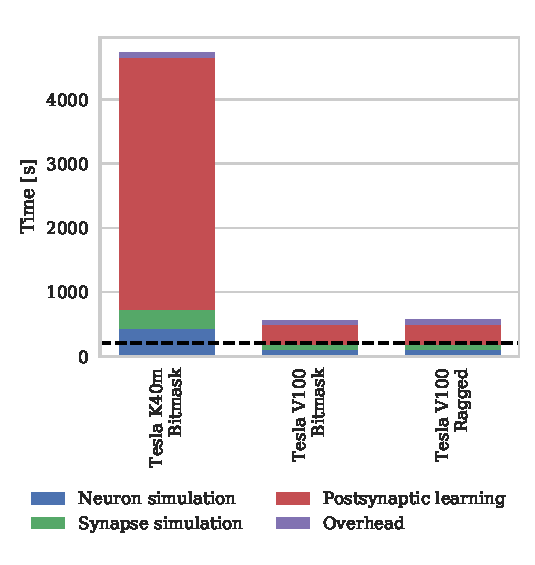
\includegraphics[width=85mm]{figures/stdp_performance}
    \end{center}
    \caption{Simulation times of balanced random network model running on various GPU hardware for \SI{200}{\second} of biological time.
    `Overhead' in GPU simulations refers to time spent in simulation loop but not within CUDA kernels.}
    \label{fig:stdp_performance}
\end{figure}

Figure~\ref{fig:stdp_performance} shows the runtime of simulations of the balanced random network model described in section~\ref{sec:method/balanced_random}.
While the simulations of the cortical microcircuit model ran approximately twice as fast on the newer Tesla V100 GPU -- potentially simply reflecting its higher memory bandwidth -- the simulations of the plastic model ran more than $10\times$ faster on the V100 GPU due almost entirely to the postsynaptic learning kernel.
This kernel is where synaptic potentiation is applied using the approach outlined in section~\ref{sec:method/balanced_random} in which an additional column-wise sparse matrix structure is used to select weights to update in response to postsynaptic spikes.
We believe that two new features of the Volta architecture~\citep{Nvidia2017} used by the V100 GPU are playing a crucial role in accelerating this process.
Firstly, Volta GPUs have \SI{6144}{\kibi\byte} of L2 cache compared to only \SI{1536}{\kibi\byte} in the older Kepler architecture used by the Tesla K40c.
This helps overcoming the cost of the non-coalesced accesses to synaptic weights.
Additionally, Volta GPUs can now simultaneously execute integer and floating point operations, meaning that the pointer arithmetic required to calculate the indices into the synaptic weight matrix can be performed simultaneously with the actual learning rule update.

\subsection{Power and energy}
\begin{figure}
    \begin{center}
        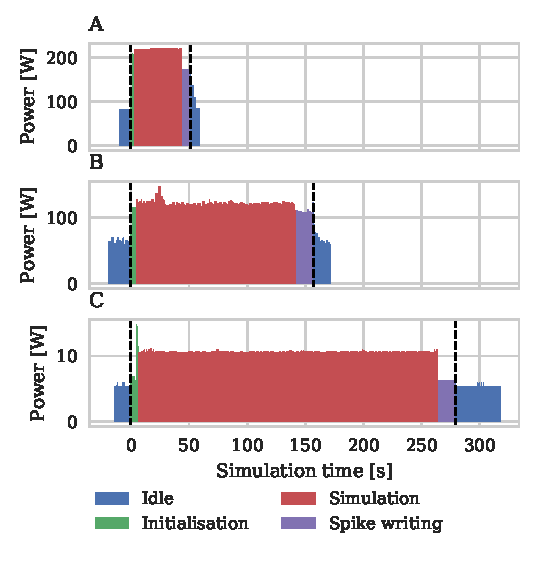
\includegraphics[width=85mm]{figures/microcircuit_power}
    \end{center}
    \caption{Power consumption during \SI{10}{\second} microcircuit simulation.
    Power was measured using consumer power measurement device with minimum resolution of \SI{0.1}{\watt} at mains socket.\\
    \textbf{(A)} Tesla K40c in a workstation with a Intel Xeon E5-1620 v2 processor running Ubuntu 16.04 LTS.\\
    \textbf{(B)} GeForce 1050Ti in a desktop PC with an Intel Core i5 750 processor running Windows 7.\\
    \textbf{(C)} NVIDIA Jetson TX2 development kit running Ubuntu 16.04 LTS and JetPack 3.2.1 in maximum performance mode.}
    \label{fig:microcircuit_power}
\end{figure}

As well as recording the runtimes of the microcircuit benchmark described in the previous section, we also recorded the power usage of the systems being benchmarked using a consumer power measurement device at the mains socket.
The screen of the power measurement device was recorded using a webcam, optical character recognition was performed using `Seven Segment Optical Character Recognition' developed by \citet{Auerswald2018} and the resultant power measurements were tagged with a time and written to disk.
Figure~\ref{fig:microcircuit_power} shows the power usage over time for simulations of the microcircuit model running for \SI{10}{\second} of biological time on each of the devices listed in table~\ref{tab:gpu_devices} aside from the Tesla V100 to which we do not have local access.

\begin{table}
  \centering
  \begin{tabular}{r S S S}
    \toprule
        {Model}                 & {Energy to solution}      & {Simulation energy}       & {Energy per synaptic event} \\
                                & {[\si{\kilo\watt\hour}]}  & {[\si{\kilo\watt\hour}]}  & {[\si{\micro\joule}]} \\
    \midrule
        GeForce 1050 Ti         & 0.0053                    & 0.0051                    & 2.0 \\
        Jetson TX2              & 0.00080                   & 0.00078                   & 0.30  \\
        Tesla K40c              & 0.0030                    & 0.0028                    & 1.08 \\
        SpiNNaker               & {--}                      & 0.017                     & 5.9 \textsuperscript{1}\\
        NEST (lowest energy)    & {--}                      & 0.012                     & 4.4 \\
    \bottomrule
  \end{tabular}

  \caption{Energy cost of simulations.
  Energy to solution and simulation energy of GPU are calculated using the \lstinline{numpy.trapz} and the simulation energy is divided by the total number of synaptic events processed to obtain the energy per synaptic event.
  For comparison, simulation energies for SpiNNaker and the NEST simulation with the lowest simulation energy (2 nodes) are read off the figure presented by \citet{VanAlbada2018}.
  Energies per synaptic event for SpiNNaker and the NEST are those reported by \citet{VanAlbada2018}.\\
  \textsuperscript{1}~This energy per synaptic event is calculated after the `idle' power of the SpiNNaker system has been taken into account.}
  \label{tab:energy_measures}
\end{table}

By integrating the power time series using the \lstinline{numpy.trapz} function we then calculated the energy to solution for each device as well as the energy per synaptic event -- a common measure for comparing the energy efficiency of neuromorphic systems.
These energy costs are listed in table~\ref{tab:energy_measures} alongside the energy costs presented by \citet{VanAlbada2018} for simulations running on SpiNNaker and a CPU-based cluster.
Whilst we were unable to measure the energy of the Tesla V100 system directly, Tesla GPUs have built in power monitoring which shows that the Tesla V100 drew a maximum of \SI{88}{\watt} compared to \SI{107}{\watt} for the Tesla K40c.
As the workstation containing the Tesla K40c drew \SI{218}{\watt} while simulating the model, compared to an idle power draw of \SI{84}{\watt}, we can estimate that the single CPU core being used by the simulation was drawing \SI{27}{\watt} more than when the system was idle.
Therefore we can estimate that, if a Tesla V100 was attached to the same workstation, the maximum power draw would be reduced to \SI{199}{\watt} suggesting that, based on the reduced simulation time of \SI{22}{\second}, the simulation energy for such a system would be \SI{0.0012}{\kilo\watt\hour} and the energy per synaptic event would be \SI{0.47}{\micro\joule}.

From figure~\ref{fig:microcircuit_power} we can see that even an idling workstation draws on the order of \SI{100}{\watt} and, as \citeauthor{VanAlbada2018} discusses, a single infiniband switch has a TDP of over \SI{200}{\watt}.
Therefore it is somewhat unsurprising that any accelerator that allows equivalent simulations to be run on fewer nodes would significantly improve energy usage.
Furthermore, as \citeauthor{VanAlbada2018} discusses, slowing SpiNNaker simulations down to this degree and simulating so few neurons on each processor results in very poor energy efficiency.
However, in a previous study using a much smaller cortical microcircuit model suffering from none of these issues, \citet{Sharp2012} measured the power usage of a SpiNNaker system and found energy usage corresponding to \SI{0.11}{\micro\joule} per synaptic event.
This suggests that although, even fully-programmable neuromorphic systems such as SpiNNaker use less energy than the most energy-efficient GPU, this is only by a margin of around $3-5\times$ when compared to newer GPUs such as the Tesla V100 and the Jetson TX2.

\section{Discussion}
\subsection{Neurorobotics}
\label{sec:discussion/neurobotics}
Neurorobotics involves the development of robots with controllers inspired by the brain, allowing neural function to be studied in an embodied context.
Neuro robots have been developed with controllers inspired by the mammalian Hippocampus~\citep{Krichmar2005} as well as the honey bee~\citep{Cope2016} and other insects~\citep{Blanchard2000}.
However computational constraints have meant that these systems have either had to be operated in simulation or that their brain-inspired controllers have had to be simulated externally to the robot. \todo{latency}

The low power requirements and real-time performance of neuromorphic systems make them obvious candidate for building neuro robotics controllers.
However, in order to interface with the robot's hardware and convert sensor data into spike trains, these systems typically need to be accompanied by a standard CPU.
For example, \citet{Kreiser2018} developed a path integration model on the Dynapse~\citep{Qiao2015} neuromorphic system which used a Parallela~\citep{Olofsson2015} board to interface with the robot and \citet{Hwu2017} developed a self-driving robot using a spiking convolutional neural network running on a TrueNorth NS1e development board which includes a Zynq SoC~\todo{cite}.
While both the Dynapse and TrueNorth systems have a negligible power consumption, the NS1e development board draws between \SIrange{2}{3}{\watt}~\citep{Sawada2016} and the Parallela \SI{5}{\watt}, somewhat out-weighing their theoretical advantages over embedded GPUs such as the Jetson TX2 which draws a maximum of \SI{15}{\watt}.

Because SpiNNaker is based on programmable ARM cores which can be used to interface with robot hardware it can be directly interfaced with a variety of robots developed at the Technical University of Munich~\citep{Denk2013}.
However, the 48 chip SpiNNaker board used on the robot developed by \citeauthor{Conradt2015} is around $10\times$ larger than a Jetson TX2, restricting its use to large ground-based robots whereas the Jetson TX2 is small and light enough to be used on both ground and aerial robots.

\subsection{Further optimisation and GPU architectures}
Because GPUs architectures do not require the complex centralized structures such as coherent caches which makes simply adding more CPU cores to symmetric multiprocessors difficult~\todo{citation}, it is expected that GPU hardware will continue to scale~\todo{citation}.
However, when simulating SNNs, a GPU's performance is likely to be constrained by its memory bandwidth.
Although upcoming technologies such as third generation High Bandwidth Memory~(HBM3) are likely to offer increases in memory bandwidth in the future, alternative strategies are still going to be required to better utilise current GPUs for SNN simulation as well as to increase the size of models that can be simulated using embedded GPUs such as the Jetson TX2 in the type of neurorobotic applications discussed in section~\ref{sec:discussion/neurobotics}.

As we discussed in the introduction, the computational requirements of training Artificial Neural Networks~(ANNs) of ever-increasing size and complexity has been a major driver in the development of GPU hardware.\todo{cite}
These applications and the growing need to deploy ready-trained ANNs to perform inference in real time on low-power `edge computing' devices mean that, here to, available memory bandwidth is beginning to limit performance.
One solution has been to use lower precision \SI{16}{\bit} floating point and even fixed point integer representations for weights~\citep{Micikevicius2017}.
Using smaller data types not only saves memory and memory bandwidth but, on some newer GPU hardware including the Jetson TX2, each CUDA thread can perform four \SI{8}{\bit} or two \SI{16}{\bit} operations simultaneously -- significantly increasing peak performance.
While lower precision types are unlikely to provide enough numerical stability for storing neuron state variables, as discussed by \citet{VanAlbada2018}, the \SI{16}{\bit} synaptic weights used by SpiNNaker provide sufficient accuracy for the microcircuit model described in section~\ref{sec:method/microcircuit}.
GeNN does not currently support these lower-precision types, but we plan on extending the algorithms described in section~\ref{sec:method} to support \SI{16}{\bit} floating point synaptic weights which should offer a significant performance improvement while not sacrificing the flexibility of floating point programming.

In this paper we have only considered single GPU simulations of circuit-scale SNN models.
However, using supercomputer systems, models with around a billion neurons can now be simulated~\citep{Jordan2018} and computational neuroscientists are beginning to use this capability to investigate the interactions between multiple circuit-scale models.
For example, \citet{Schmidt2015} developed a model of the Macaque visual cortex consisting of 32 cortical areas, each modelled as a customised version of the model described in section~\ref{sec:method/microcircuit}.
Even if half-precision floating point weights were employed, a single GPU would not have enough memory to store such a model.
However, systems such as the NVIDIA DGX-2~\todo{cite} are now available which contain several Tesla V100 GPUs, connected through a crossbar with a \SI{900}{\giga\byte\per\second} bisection bandwidth.
While GeNN does not currently target such multi-GPU systems, because the GPUs in such a system are still all connected to a single host system, many of the advantages of GPU simulations \todo{finish}
Beyond this scale, an additional level of parallelism could be achieved using MPI to distribute GPU-accelerated simulations across multiple HPC nodes.
While, the communication latencies would , NVIDIA's GPUDirect~\todo{cite} technology allows data to be transferred directly between GPUs via compatible network cards rather than having to go via the host computers main memory.

\subsection{Interactive simulation}
As discussed in the introduction, one of the major uses of SNN simulations in computational neuroscience is for characterising and exploring the subset of model's parameter space left under-constrained by experimental data.

In common with many other application areas, computational neuroscience simulations are typically performed in a non-interactive `batch' mode in which a simulation is started (either on a remote HPC system or locally) and some time later results are returned.
The results of such simulations are then analysed offline to determine whether a particular combination of parameters has resulted in a meaningful\todo{correct word} result.
However, it is difficult to determine what data will be required for this analysis ahead of time.
Recording too much data requires large amounts of disk space and potentially slows down both the simulation and analysis.
One solution to this problem is \textit{Computational steering}~\citep{Parker1997} -- a technology that allows researchers to change the parameters of a running simulation as well as which state variables are being visualised.
With the development of large-scale models such as those discussed in the previous section, the need for approaches such as computation steering in computational neuroscience is becoming apparant.

\citet{Nowke2018} developed a computational steering system for visualising and steering NEST simulations.
However, when running this system across a CPU-based HPC system, \citeauthor{Nowke2018} found that its scalability was dictated by the amount of data that had to be transferred across the network at each simulation timestep.
The next generation of supercomputer systems are being designed specifically to address these issues~\cite{Lippert2014}.
However, as discussed in section~\ref{sec:discussion/neurobotics}, GPUs are much more suited to this type of tight interaction between visualisation and simulation as they exist within the host system's memory space allowing data to be exchanged at the speed of the PCI express bus rather than an external network.
Additionally, because CUDA can interact directly with graphics APIs such as OpenGL, some simple visualisations could be rendered without any interaction with the host computers CPU at all.

\section*{Conflict of Interest Statement}
The authors declare that the research was conducted in the absence of any commercial or financial relationships that could be construed as a potential conflict of interest.

\section*{Author Contributions}
JK and TN wrote the paper.
TN is the original developer of GeNN.
JK is currently the primary GeNN developer and was responsible for extending the code generation approach to the parallel initialisation of networks.
JK performed the experiments and the analysis of their results which are presented in this work.

\section*{Funding}
This work was funded by the EPSRC (Brains on Board project, grant number EP/P006094/1).

\section*{Acknowledgments}
We would like to thank Andrew Webb for his thoughts on efficient parallel connectivity generation.
We would also like to thank Sacha van Albada for providing the data from her NEST simulations and clarifying some parts of the accuracy analysis -- without these contributions section~\ref{sec:results/correctness} would not have been possible.
This is a short text to acknowledge the contributions of specific colleagues, institutions, or agencies that aided the efforts of the authors.

\section*{Data Availability Statement}
The datasets [GENERATED/ANALYZED] for this study can be found in the [NAME OF REPOSITORY] [LINK].
% Please see the availability of data guidelines for more information, at https://www.frontiersin.org/about/author-guidelines#AvailabilityofData
%
\bibliographystyle{frontiersinSCNS_ENG_HUMS}
\bibliography{frontiers_genn}

%%% Make sure to upload the bib file along with the tex file and PDF
%%% Please see the test.bib file for some examples of references

\end{document}
